\documentclass[final]{fhnwreport}       %[mode] = draft or final
                                        %{class} = fhnwreport, article, 
                                        %          report, book, beamer, standalone

%%---Main Packages-----------------------------------------------------------------------
\usepackage[english, ngerman]{babel}	%Mul­tilin­gual sup­port for LaTeX
\usepackage[T1]{fontenc}				%Stan­dard pack­age for se­lect­ing font en­cod­ings
\usepackage[utf8]{inputenc}				%Ac­cept dif­fer­ent in­put en­cod­ings
\usepackage{lmodern}                    %The newer Font-Set
\usepackage{textcomp}					%LaTeX sup­port for the Text Com­pan­ion fonts
\usepackage{graphicx} 					%En­hanced sup­port for graph­ics
\usepackage{float}						%Im­proved in­ter­face for float­ing ob­jects
\usepackage{ifdraft}                    %Let you check if the doc is in draft mode

%%---Useful Packages---------------------------------------------------------------------
\usepackage[pdftex,dvipsnames]{xcolor}  %Driver-in­de­pen­dent color ex­ten­sions for LaTeX
\usepackage{csquotes}                   %Simpler quoting with \enquote{}
\usepackage{siunitx} 					%A com­pre­hen­sive (SI) units pack­age
\usepackage{listings}					%Type­set source code list­ings us­ing LaTeX
\usepackage[bottom]{footmisc}			%A range of foot­note op­tions
\usepackage{footnote}					%Im­prove on LaTeX's foot­note han­dling
\usepackage{verbatim}					%Reim­ple­men­ta­tion of and ex­ten­sions to LaTeX ver­ba­tim
\usepackage[textsize=footnotesize]{todonotes} %Mark­ing things to do in a LaTeX doc­u­ment

%%---Tikz Packages-----------------------------------------------------------------------
\usepackage{standalone}
\usepackage{tikz}
\usepackage{circuitikz}
\usetikzlibrary{arrows}
\usetikzlibrary{calc}
\usetikzlibrary{intersections}

%%---Math Packages-----------------------------------------------------------------------
\usepackage{amsmath}					%AMS math­e­mat­i­cal fa­cil­i­ties for LaTeX
%\usepackage{amssymb}					%Type­set­ting symbols (AMS style)
%\usepackage{array}						%Ex­tend­ing the ar­ray and tab­u­lar en­vi­ron­ments
%\usepackage{amsthm}					%Type­set­ting the­o­rems (AMS style)

%%---Table Packages----------------------------------------------------------------------
\usepackage{tabularx}					%Tab­u­lars with ad­justable-width columns
%\usepackage{longtable}
\usepackage{multirow}					%Create tab­u­lar cells span­ning mul­ti­ple rows
\usepackage{multicol}					%In­ter­mix sin­gle and mul­ti­ple columns

%%---PDF / Figure Packages---------------------------------------------------------------
\usepackage{pdfpages}					%In­clude PDF doc­u­ments in LaTeX
\usepackage{pdflscape}					%Make land­scape pages dis­play as land­scape
\usepackage{subfig}					    %Fig­ures di­vided into sub­fig­ures
\usepackage{placeins}                   % use \FloatBarrier to restrict float behind this place

%%---Other Packages----------------------------------------------------------------------
%\usepackage{xargs}                     %De­fine com­mands with many op­tional ar­gu­ments

%%---Bibliography------------------------------------------------------------------------
\usepackage[style=ieee,urldate=comp,backend=biber]{biblatex}
\addbibresource{literature/bibliography.bib}

%%---Main Settings-----------------------------------------------------------------------
\graphicspath{{./graphics/}}			%Defines the graphicspath
%\geometry{twoside=false}				    %twoside=false disables the "bookstyle"
\setlength{\marginparwidth}{2cm}
%\overfullrule=5em						%Creates a black rule if text goes over the margins => debugging


%%---User Definitions--------------------------------------------------------------------
%%Tabel-Definitions: (requires \usepackage{tabularx})
\newcolumntype{L}[1]{>{\raggedright\arraybackslash}p{#1}}    %column-width and alignment
\newcolumntype{C}[1]{>{\centering\arraybackslash}p{#1}}
\newcolumntype{R}[1]{>{\raggedleft\arraybackslash}p{#1}}

%%---Optional Package Settings-----------------------------------------------------------
%Listings-Settings: (requires \usepackage{listings}) => Example with Matlab Code
\lstset{language=Matlab,%
    basicstyle=\footnotesize\ttfamily,
    breaklines=false,%
    morekeywords={switch, case, otherwise},
    keywordstyle=\color{Blue},%
    tabsize=2,
    %morekeywords=[2]{1}, keywordstyle=[2]{\color{black}},
    identifierstyle=\color{Black},%
    stringstyle=\color{Purple},
    commentstyle=\color{Green},%
    showstringspaces=false,%without this there will be a symbol in the places where there is a space
    numbers=left,%
    numberstyle={\tiny \color{black}},% size of the numbers
    numbersep=9pt, % this defines how far the numbers are from the text
    %emph=[1]{word1, word2,...},emphstyle=[1]\color{red}
}				

%%---Projectspecific------------------------------------------------------------------------
\usepackage{pgfplots}	
%\usepackage{IEEEtrantools}	
%\usepackage{array}
%\usepackage{lipsum}
%\usepackage{etoolbox}
%\usepackage{setspace}
\usetikzlibrary{shapes,decorations.markings,backgrounds,patterns}
\usepackage[framed,numbered,autolinebreaks,useliterate]{mcode}

%%%
%%% For the SFGs
%%%
\tikzset{%
% Style of the node
    Node/.style={circle,thick,draw=black,inner sep=0, minimum size=0.15cm},
    Start/.style={draw=red},
    End/.style={draw=blue},
    Interm/.style={},
% Style of the node label
    NodeName/.style={font=\footnotesize,black, outer sep=1},
    NodeName n/.style={NodeName, above},
    NodeName s/.style={NodeName, below},
    NodeName e/.style={NodeName, right},
    NodeName w/.style={NodeName, left},
% Style of the branche label
    ArrowName/.style={font=\footnotesize,auto,outer sep=1},
    ArrowName n/.style={ArrowName, above},
    ArrowName s/.style={ArrowName, below},
    ArrowName e/.style={ArrowName, right},
    ArrowName w/.style={ArrowName, left},
% Style of the branch
    Connection/.style={thick},
    NodeBezier/.style={},
    ->-/.style={decoration={
        markings,
        %mark=at position #1 with {\arrow[scale=1.3,shorten >=1cm]{>}}},
        mark=at position #1 with {\draw[->,>=latex',ultra thick](0pt,0)--(4pt,0);}},
        postaction={decorate}},
    ->-/.default=0.50,
}

% Engineering

\makeatletter

\newif\ifpgfplots@scaled@x@ticks@engineering
\pgfplots@scaled@x@ticks@engineeringfalse
\newif\ifpgfplots@scaled@y@ticks@engineering
\pgfplots@scaled@y@ticks@engineeringfalse
\newif\ifpgfplots@scaled@z@ticks@engineering
\pgfplots@scaled@z@ticks@engineeringfalse

\pgfplotsset{
    scaled x ticks/engineering/.code=
        \pgfplots@scaled@x@ticks@engineeringtrue,
    scaled y ticks/engineering/.code=
        \pgfplots@scaled@y@ticks@engineeringtrue,
    scaled z ticks/engineering/.code=
        \pgfplots@scaled@y@ticks@engineeringtrue,
%    scaled ticks=engineering  % Uncomment this line if you want "engineering" to be on by default
}

\def\pgfplots@init@scaled@tick@for#1{%
    \global\def\pgfplots@glob@TMPa{0}%
    \expandafter\pgfplotslistcheckempty\csname pgfplots@prepared@tick@positions@major@#1\endcsname
    \ifpgfplotslistempty
        % we have no tick labels. Omit the tick scale label as well!
    \else
    \begingroup
    \ifcase\csname pgfplots@scaled@ticks@#1@choice\endcsname\relax
    % CASE 0 : scaled #1 ticks=false: do nothing here.
    \or
        % CASE 1 : scaled #1 ticks=true:
        %--------------------------------
        % the \pgfplots@xmin@unscaled@as@float  is set just before the data
        % scale transformation is initialised.
        %
        % The variables are empty if there is no datascale transformation.
        \expandafter\let\expandafter\pgfplots@cur@min@unscaled\csname pgfplots@#1min@unscaled@as@float\endcsname
        \expandafter\let\expandafter\pgfplots@cur@max@unscaled\csname pgfplots@#1max@unscaled@as@float\endcsname
        %
        \ifx\pgfplots@cur@min@unscaled\pgfutil@empty
            \edef\pgfplots@loc@TMPa{\csname pgfplots@#1min\endcsname}%
            \expandafter\pgfmathfloatparsenumber\expandafter{\pgfplots@loc@TMPa}%
            \let\pgfplots@cur@min@unscaled=\pgfmathresult
            \edef\pgfplots@loc@TMPa{\csname pgfplots@#1max\endcsname}%
            \expandafter\pgfmathfloatparsenumber\expandafter{\pgfplots@loc@TMPa}%
            \let\pgfplots@cur@max@unscaled=\pgfmathresult
        \fi
        %
        \expandafter\pgfmathfloat@decompose@E\pgfplots@cur@min@unscaled\relax\pgfmathfloat@a@E
        \expandafter\pgfmathfloat@decompose@E\pgfplots@cur@max@unscaled\relax\pgfmathfloat@b@E
        \pgfplots@init@scaled@tick@normalize@exponents
        \ifnum\pgfmathfloat@b@E<\pgfmathfloat@a@E
            \pgfmathfloat@b@E=\pgfmathfloat@a@E
        \fi
        \xdef\pgfplots@glob@TMPa{\pgfplots@scale@ticks@above@exponent}%
        \ifnum\pgfplots@glob@TMPa<\pgfmathfloat@b@E
            % ok, scale it:
            \expandafter\ifx % Check whether we're using engineering notation (restricting exponents to multiples of three)
                \csname ifpgfplots@scaled@#1@ticks@engineering\expandafter\endcsname
                \csname iftrue\endcsname
                    \divide\pgfmathfloat@b@E by 3
                    \multiply\pgfmathfloat@b@E by 3
            \fi
            \multiply\pgfmathfloat@b@E by-1
            \xdef\pgfplots@glob@TMPa{\the\pgfmathfloat@b@E}%
        \else
            \xdef\pgfplots@glob@TMPa{\pgfplots@scale@ticks@below@exponent}%
            \ifnum\pgfplots@glob@TMPa>\pgfmathfloat@b@E
                % ok, scale it:
                \expandafter\ifx % Check whether we're using engineering notation (restricting exponents to multiples of three)
                    \csname ifpgfplots@scaled@#1@ticks@engineering\expandafter\endcsname
                    \csname iftrue\endcsname
                        \advance\pgfmathfloat@b@E by -2
                        \divide\pgfmathfloat@b@E by 3
                        \multiply\pgfmathfloat@b@E by 3
                \fi
                \multiply\pgfmathfloat@b@E by-1
                \xdef\pgfplots@glob@TMPa{\the\pgfmathfloat@b@E}%
            \else
                % no scaling necessary:
                \xdef\pgfplots@glob@TMPa{0}%
            \fi
        \fi
    \or
        % CASE 2 : scaled #1 ticks=base 10:
        %--------------------------------
        \c@pgf@counta=\csname pgfplots@scaled@ticks@#1@arg\endcsname\relax
        %\multiply\c@pgf@counta by-1
        \xdef\pgfplots@glob@TMPa{\the\c@pgf@counta}%
    \or
        % CASE 3 : scaled #1 ticks=real:
        %--------------------------------
        \pgfmathfloatparsenumber{\csname pgfplots@scaled@ticks@#1@arg\endcsname}%
        \global\let\pgfplots@glob@TMPa=\pgfmathresult
    \or
        % CASE 4 : scaled #1 ticks=manual:
        \expandafter\global\expandafter\let\expandafter\pgfplots@glob@TMPa\csname pgfplots@scaled@ticks@#1@arg\endcsname
    \fi
    \endgroup
    \fi
    \expandafter\let\csname pgfplots@tick@scale@#1\endcsname=\pgfplots@glob@TMPa%
}
\makeatother			                %loads all packages, definitions and settings												
\title{Antennensimulationen in CST - Bericht hf1}          %Project Title
\author{Simon Zoller, Thomas Frei}          %Document Type => Technical Report, ...
\date{Windisch, \today}             %Place and Date


\begin{document}

%%---TITLEPAGE---------------------------------------------------------------------------
\selectlanguage{english}                %ngerman or english
\maketitle

\vspace*{-1cm}						    %compensates the space after the date line.
\vfill
%\begin{figure}[H]
%\centering
%\includegraphics[width=\linewidth]{titelbild.pdf}
%\end{figure}
\vfill

{
\renewcommand\arraystretch{2}
\begin{center}
\begin{tabular}{>{\bf}p{4cm} l}
Universität                &    Fachhochschule Nordwestschweiz\\
Studiengang                &    Elektro- und Informationstechnik\\
Autor   		           & 	Simon Zoller, Thomas Frei\\
Betreuer                   &    Christoph Wildfeuer und Peter Niklaus\\
Version                    &    1.0 %Normally not used!
\end{tabular}
\end{center}
}

\clearpage
			
%%---ABSTRACT----------------------------------------------------------------------------
\selectlanguage{english}				%ngerman or english
\thispagestyle{empty}
\include{sections/abstract}

%%---TABLE OF CONTENTS-------------------------------------------------------------------
\pagenumbering{Roman}		
\selectlanguage{english}				%ngerman or english
\tableofcontents
\clearpage

%%---TEXT--------------------------------------------------------------------------------
\pagenumbering{arabic}
\section{Einleitung}

Ein grosses Thema der Hochfrequenztechnik sind Antennen. Generell können Antennen als Leiter angesehen werden, welche identisch zur Leitungstheorie gelten. Jedoch gibt es viele verschiedene Ausführungen welche sich alle unterschiedlich verhalten. Während des Unterrichtes wurden keine Antennen angeschaut, weshalb sich mit diesem Bericht die Möglichkeit angeboten hat, diesen Teilbereich aufzuarbeiten. Hierfür wurden im Simulationsprogramm CST Messungen ausgewählter Antennen durchgeführt, welche sich vor allem auf die Direktivität der Antennen beziehen. Als Abschluss wurde noch eine Kleeblatt Antenne modelliert, mit welcher am Institut gearbeitet wird. Zu jeder Antenne wurde zuerst die Theorie behandelt und anschliessend die entsprechenden Simulationen durchgeführt. Die Theorie wurde nach dem Buch von K. Kark aufgearbeitet \cite{book}.
\section{Dipole}

Als erstes Thema werden Dipolantennen beschrieben. Dabei wird vor allem auf den Hertzschen Dipol eingegangen, welcher das Modell der Antenne vereinfacht.

\subsection{Hertzscher Dipol}

Eine Dipol Antenna kann als kurzer Linearstrahler beschrieben werden, wobei dessen länge $l \ll \lambda_0 /4$ beträgt. $\lambda_0$ beschreibt dabei die Wellenlänge, welche durch das Verhältnis der Lichtgeschwindigkeit zur Signalfrequenz $c_0/f$ beschreibt. 

xxx

Ein solcher Strahler ist in Abbildung xxx zu sehen, wobei $\underline{I}$ der komplexe Strom einer Sinusschwingung darstellt, welche konstant über die gesamte Länge schwingt. $\phi$ stellt den Winkel dar, welcher um die z-Achse rotiert und über die x- und y-Achse aufgespannt ist.$\theta$ hingegen rotiert um die x-Achse und wird über die y- und z-Achse aufgespannt. Für die Kugelkoordinaten bedeutet dies, dass mit den Restriktionen 

\begin{align}
&0 \leq \varphi \leq 2\pi\\
&0 \leq \vartheta \leq \pi
\end{align}

der gesamte Bereich des Koordinatensystems abgedeckt ist. Das durch den Strom induzierte Magnetfeld kann mit 

\begin{equation}
\underline{H}_0 = j\pi \frac{\underline{I}l}{{\lambda_0}^2}
\end{equation}

beschrieben werden, was für zwei Formeln für das magnetische und elektrische Feld liefert:

\begin{align}
\underline{H}_\varphi   &= \underline{H}_0 \sin \vartheta \frac{e^{-jk_0r}}{k_0r}\\
\underline{E}_\vartheta &= Z_0 \underline{H}_\varphi = Z_0 \underline{H}_0 \sin \vartheta \frac{e^{-jk_0r}}{k_0r}.
\end{align}

Hierbei beschreibt $r$ die Distanz des Punktes zu Ursprung und $k_0 = \omega \sqrt{\mu_0 \eta_0} = c_0/\omega$ die Wellenzahl im Vakuum beschreibt. Somit beschreibt die komplexe Exponentialfunktion die Ausbreitung der Welle, was mit der Theorie der Wellenleitern übereinstimmt. Im Nenner ist das Abklingen des Sinus zu erkennen, welches abhängig von der Distanz zum Ursprung und der Wellenzahl ist. xxx


\subsection{Richtdiagramm}

Ein wichtiges Diagramm für die Analyse von Antennen ist das Richtdiagramm. Mit diesem kann die Direktivität einer Antenne dargestellt werden, welche mitteilt, in welche Richtung wie viel der Leistung der Antenne abgestrahlt wird. Diese Analyse geschieht im Fernfeld, was bedeutet dass die Annahme $r \rightarrow \inf$ getroffen wird.

Im Fernfeld nimmt die Krümmung der sphärischen Phasenfront einer Kugelwelle immer weiter
ab. Für r   kann die Kugelwelle lokal durch eine homogene ebene Welle angenähert werden. Die transversalen Feldkomponenten werden phasengleich und es wird nur in radialer Richtung Wirkleistung transportiert, deren Winkelverteilung durch die Sendeantenne festgelegt ist.
Der Winkelabhängigkeit der Strahlung, d.h. der Strahlungsverteilung im Raum, kommt eine
große praktische Bedeutung zu. Von ihr hängt es ab, welcher Anteil der ausgestrahlten Leistung
für den eigentlichen Verwendungszweck ausgenutzt werden kann. Strahlung in oder Aufnahme
aus unerwünschten Richtungen erhöht die gegenseitigen Störungsmöglichkeiten. Bestimmte
Aufgaben verlangen vielfach auch eine ganz bestimmte Verteilung des Strahlungsfeldes. Einen
Überblick über die Verteilung der Strahlung in verschiedene Raumrichtungen liefert die Verteilung der Fernfeldstärke einer Antenne in Abhängigkeit von der Raumrichtung   , . 
\section{Linearantennen}

Eine Linearantenne ist ein Typ Antenne, welche eine Länge um die Grösse $\lambda_0/2$ besitzt. Diese werden umgänglich für Mittel- und Langwellen Anwendungen gebraucht wegen ihrer Einfachheit. 

\subsection{Theorie}\label{sec:LinTheo}

Die Antenne besteht aus einem geraden, zylindrischen Leiter, welcher einen dünnen Durchmesser besitzt. Dabei gilt, dass der Schlankheitsgrad

\begin{equation}
s = \frac{l}{d}=\frac{2h}{d} \geq 75
\end{equation} 

beträgt und der Durchmesser

\begin{equation}
d \leq \frac{\lambda_0}{50}
\end{equation}

erfüllt. Somit kann für die Berechnung der Felder die Integration über eine Hüllfläche durch eine eindimensionale Integration vereinfacht werden, was den Rechenaufwand erleichtert.

\begin{figure}[!ht]
	\centering
    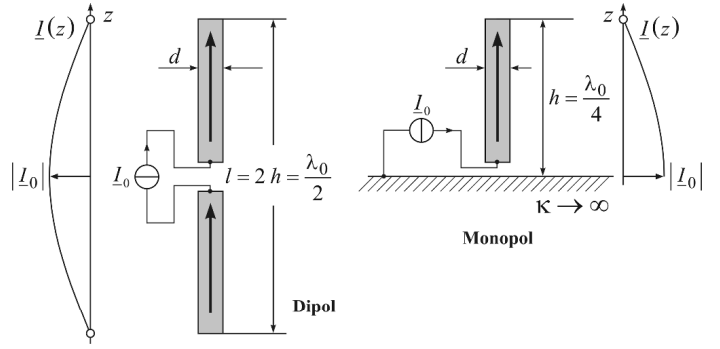
\includegraphics[width=\textwidth]{DiMonopol.png}
    \caption{Unterschiedliche Speisung von Monopol und Dipolantennen.}
    \label{fig:DiMonopol}
\end{figure}

Die lineare Antenne kann auf zwei Arten gespiesen werden. Entweder wird die Antenne als Monopol betrieben und am Fusspunkt gegen Erde erregt, oder sie wird in der Mitte als Monopol symmetrisch erregt (dargestellt in Abbildung \ref{fig:DiMonopol}). Bei der Dipol Ausführung ist jedoch ein Spalt in der Mitte notwendig, welcher vernachlässigbar klein sein soll. Die beiden Anordnungen unterscheiden sich nicht im Strahlungsdiagramm da die Erdoberfläche die Symmetrieebene des elektrischen Feldes darstellt. Der Monopol, welcher halb so lang wie der Dipol gewählt wird, gibt bei einem identischen Speisestrom gerade die halbe Strahlungsleistung ab, was zu einem doppelten Gewinn führt.\\

Für die Simulationen interessieren uns die Richtdiagramme der Linearantennen. Dazu wurde der Halbwellendipol, der Ganzwellendipol und der Doppelwellendipol betrachtet. Die Herleitung der Richtcharakteristik wurde weggelassen, da uns hauptsächlich die Simulationsresultate interessieren. Die bereits berechneten Werte wurden aus dem Buch von K. Kark entnommen \cite{book}.\\

Der Halbwellendipol besitzt eine Antennenlänge von $\lambda_0/2$, was zu einer Richtcharakteristik von 

\begin{equation}\label{eq:RichtHalb}
C(\vartheta) = \frac{\cos \left(\frac{\pi}{2}\cos \vartheta \right)}{\sin \vartheta}
\end{equation}

führt. Die Richtcharakteristik des Ganzwellendipols beträgt bei dessen Antennenlänge von $\lambda_0$

\begin{equation}
C(\vartheta) = \frac{\cos^2 \left(\frac{\pi}{2}\cos \vartheta \right)}{\sin \vartheta}.
\end{equation}

Der Doppelwellendipol ist $2\lambda_0$ lang und dessen Richtcharakteristik beträgt

\begin{equation}\label{eq:RichtDoppel}
C(\vartheta) = \frac{\sin^2 \left(\pi \cos \vartheta \right)}{\sin \vartheta}.
\end{equation}

\begin{figure}[!ht]
	\centering
    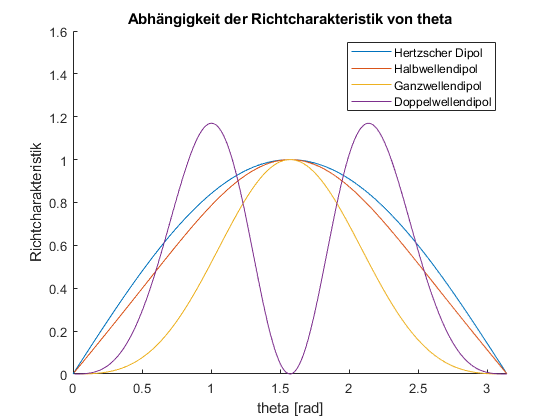
\includegraphics[width=\textwidth/4*3]{Wellendipol.png}
    \caption{Ein Plot der jeweiligen Richtcharakteristiken verschiedener Linearantennen.}
    \label{fig:Wellendipol}
\end{figure}

In Abbildung \ref{fig:Wellendipol} ist die Richtcharakteristik der Antennen in Abhängigkeit von $\vartheta$ zu sehen. Dabei wurde der Hertzsche Dipol auch eingefügt, um die Richtdiagramme besser vergleichen zu können. Wie sich erkennen lässt, besitzt der Hertzsche Dipol die grösste Halbwertsbreite von allen Antennen. Beim Halbwellendipol ist diese nur leicht kleiner, wobei sich beim Ganzwellendipol eine bemerkbar kleinere Halbwertsbreite einstellt. Dabei liegen die -3dB Punkte bei \num{1.99} und \num{1.15}, welche eine Halbwertsbreite von \SI{48}{\degree} besitzen. Diese beträgt fast halb so viel wie die \SI{90}{\degree} Halbwertsbreite des Hertzschen Dipols. Der Doppelwellendipol besitzt sogar eine Nullstelle bei $\pi/2$, wo sich die Maximalwerte der anderen Antennen befinden. Der Maximalwert des Doppelwellendipols liegt jedoch bei \num{1} und \num{2.14}, was einen Maximalwert bei \SI{57.3}{\degree} und \SI{122.6}{\degree} ergibt. Dabei wird klar, dass das dazugehörige Richtdiagramm vier Keulen besitzen wird.\\

\subsection{Simulation}

Im Buch von K. Kark auf Seite 249 befindet sich eine Tabelle mit den Richtdiagrammen der obigen genannten linearen Antennen \cite{book}. Dabei wurde die Länge der jeweiligen Antenne noch mit dem Faktor n angepasst, was uns aus den Formeln \ref{eq:RichtHalb} bis \ref{eq:RichtDoppel} folgende Längen und Richtcharakteristiken ergeben:

Für den Halbwellendipol:

\begin{align}
l &= (2n-1)\frac{\lambda_0}{2}\label{eq:l1}\\
C(\vartheta) &= \frac{\cos \left(\frac{2n-1}{2}\pi \cos \vartheta \right)}{\sin \vartheta}
\end{align} 

Für den Ganzwellendipol:

\begin{align}
l &= (2n-1)\lambda_0\label{eq:l2}\\
C(\vartheta) &= \frac{\cos^2 \left(\frac{2n-1}{2}\pi \cos \vartheta \right)}{\sin \vartheta}
\end{align} 

Für den Doppelwellendipol:

\begin{align}
l &= 2n\lambda_0\label{eq:l3}\\
C(\vartheta) &= \frac{\sin^2 \left(n \pi \cos \vartheta \right)}{\sin \vartheta}
\end{align} 

Für die Simulation wurde ein Dipol mit anpassbarer Länge aufgebaut, mit welchem zwischen den drei in den Formeln \ref{eq:l1}, \ref{eq:l2} und \ref{eq:l3} genannten Längen umgeschaltet werden kann. Für die Anregung sitzt ein Vakuum mit vernachlässigbarer Länge in der Mitte der Antenne, in welchem sich der Anregungsport befindet. Für die Simulation wurde das Standard Anregungssignal verwendet und als Frequenz wurde \SI{1}{\giga\hertz} verwendet. Die Datei wurde so geschrieben, dass alle Antennentypen mit minimalem Aufwand simuliert werden können, ohne dass das Modell abgeändert werden muss. Für alle Abbildungen wurde der Vertikalschnitt der Richtcharakteristik genommen. Es entsteht eine Rotationssymmetrie auf der Antennenachse (was in der Simulation der z-Achse entspricht).

\newpage

\begin{figure}[!ht]
	\centering
    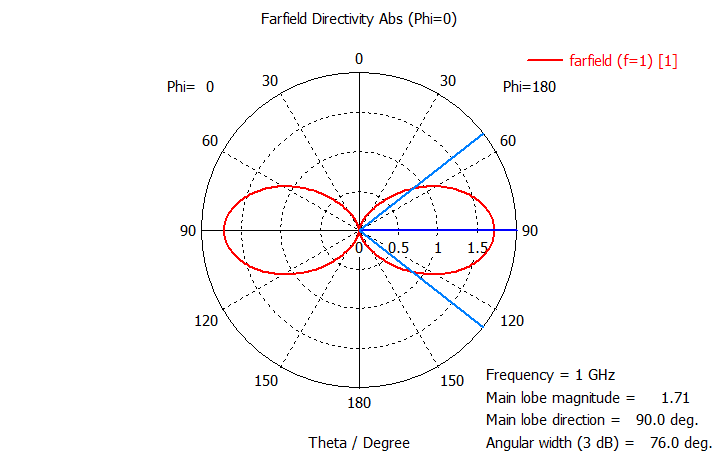
\includegraphics[width=\textwidth]{Halbwellendipol1.png}
    \caption{Direktivität der Halbwellendipolantenne.}
    \label{fig:Halbwellendipol1}
\end{figure}

In Abbildung \ref{fig:Halbwellendipol1} ist das Richtdiagramm des Halbwellendipols zu sehen. Wie bereits erwähnt ist dessen Halbwertsbreite leicht kleiner als \SI{90}{\degree} welche bei $\vartheta = 90^\circ$ am stärksten abgestrahlt wird.

\begin{figure}[!ht]
	\centering
    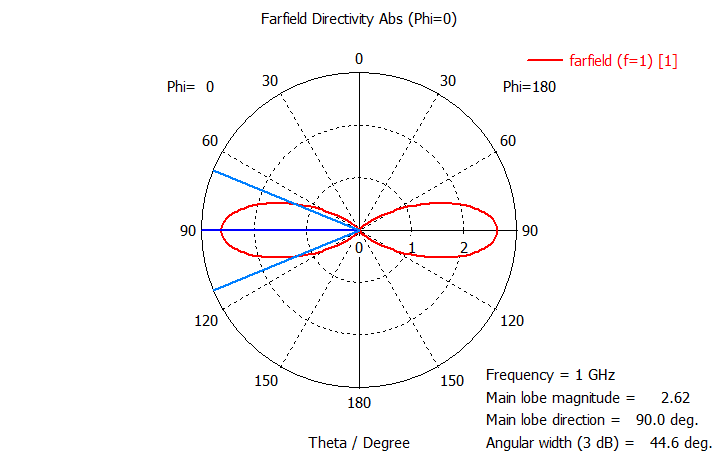
\includegraphics[width=\textwidth]{Ganzwellendipol1.png}
    \caption{Richtdiagramm des Ganzwellendipoles.}
    \label{fig:Ganzwellendipol1}
\end{figure}

Abbildung \ref{fig:Ganzwellendipol1} zeigt die Direktivität des Ganzwellendipols. Berechnet wurde dabei eine Halbwertsbreite von \SI{48}{\degree} und simuliert wurde eine Halbwertsbreite von \SI{44.6}{\degree}. Diese Abweichung ist minimal, weshalb die Simulation als erfolgreich verifiziert werden kann. Auch hier ist die Richtung der maximalen Leistungsabgabe identisch mit dem vorherigen Resultat.

\begin{figure}[!ht]
	\centering
    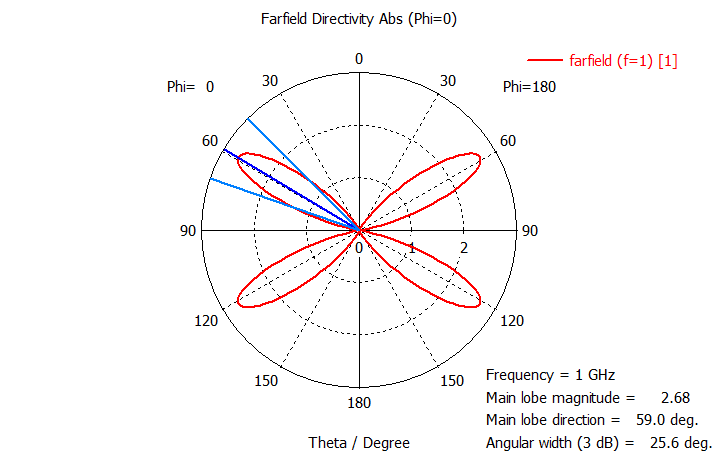
\includegraphics[width=\textwidth]{Doppelwellendipol1.png}
    \caption{Resultat der Simulation des Doppelwellendipols.}
    \label{fig:Doppelwellendipol1}
\end{figure}

Wie in Abbildung \ref{fig:Doppelwellendipol1} zu sehen ist, verhält sich das Richtdiagramm wie im Abschnitt \ref{sec:LinTheo} beschrieben wurde. Es entstehen vier Keulen, wobei der Winkel bei der Simulation \SI{59}{\degree} beträgt anstelle der berechneten \SI{57.3}{\degree}. Dies ist auch wiederum eine vernachlässigbar kleine Abweichung.\\

Als Abschluss der linearen Antenne wurden in Abbildungen \ref{fig:Halbwellendipol13} bis \ref{fig:Doppelwellendipol13} die höheren Ordnungen für $n$ simuliert. 

\newpage

\begin{figure}[!ht]
	\centering
    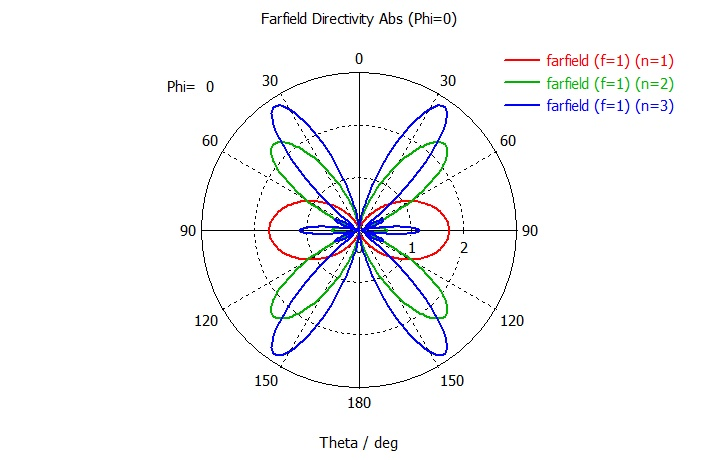
\includegraphics[width=\textwidth]{Halbwellendipol13.jpg}
    \caption{Direktivität der Halbwellendipolantenne mit $n = 1 ... 3$.}
    \label{fig:Halbwellendipol13}
\end{figure}

\begin{figure}[!ht]
	\centering
    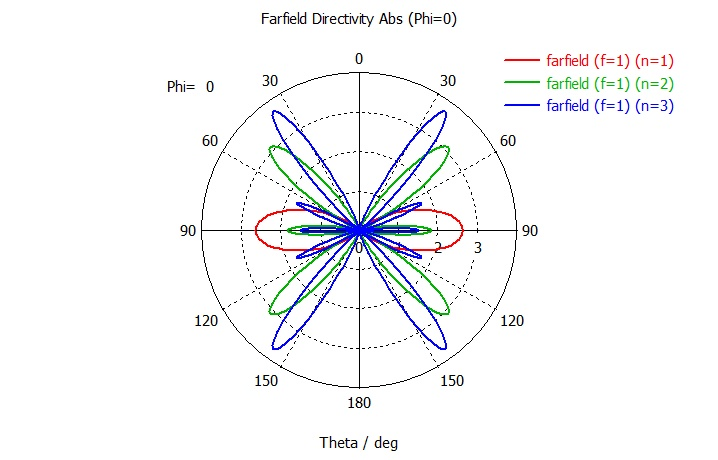
\includegraphics[width=\textwidth]{Ganzwellendipol13.jpg}
    \caption{Richtdiagramm des Ganzwellendipoles mit $n = 1 ... 3$.}
    \label{fig:Ganzwellendipol13}
\end{figure}

\newpage

\begin{figure}[!ht]
	\centering
    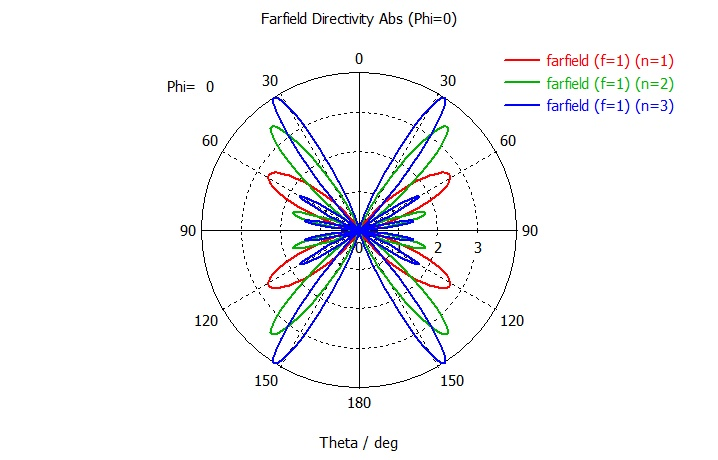
\includegraphics[width=\textwidth/10*9]{Doppelwellendipol13.jpg}
    \caption{Resultat der Simulation des Doppelwellendipols mit $n = 1 ... 3$.}
    \label{fig:Doppelwellendipol13}
\end{figure}

Die Resultate decken sich alle mit der Theorie des Fachbuches. Die Anzahl Seitenkeulen steigt identisch mit den im Fachbuch beschriebenen Abbildungen wenn die Ordnung $n$ vergrössert wird, wobei ab einer Länge grösser als $\lambda_0$ Seitenkeulen entstehen. Diese entstehen durch Überlagerungen von Beiträgen der Elementarstrahlern.

\begin{figure}[!ht]
	\centering
    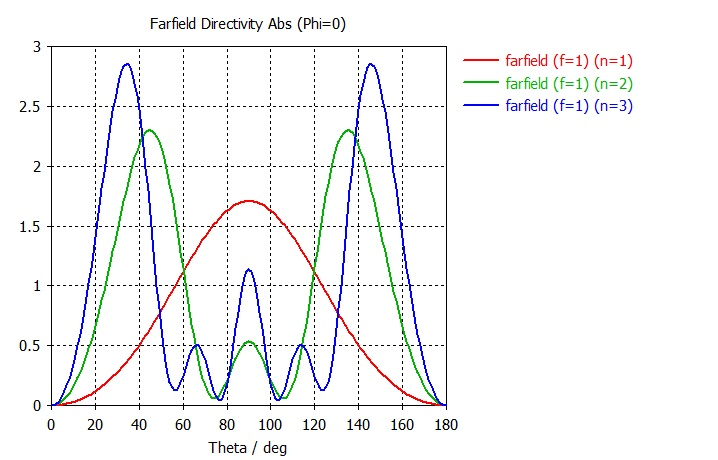
\includegraphics[width=\textwidth/10*9]{Halbwellendipol13Cart.jpg}
    \caption{Direktivität der Halbwellendipolantenne mit $n = 1 ... 3$ in kartesischen Koordinaten.}
    \label{fig:Halbwellendipol13Cart}
\end{figure}

\newpage

Natürlich kann auch im Vergleich zu Abbildung \ref{fig:Wellendipol} das Resultat in Kartesichen Koordinaten dargestellt werden. Dies resultiert in Abbildung \ref{fig:Halbwellendipol13Cart}. Somit stellt dieser Plot dasselbe Resultat wie Abbildung \ref{fig:Halbwellendipol13} dar, wobei bei den kartesischen Koordinaten das Herauslesen der Halbwertsbreite etwas einfacher ist. Bei den Kugelkoordinaten fällt es hingegen leichter, sich die Abstrahlunsrichtungen vorzustellen.

\begin{figure}[!ht]
	\centering
    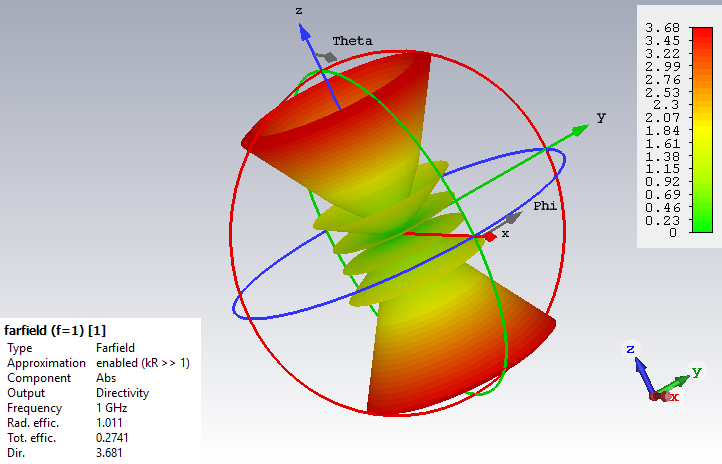
\includegraphics[width=\textwidth]{3D.png}
    \caption{Darstellung des Doppelwellendipols mit $n = 3$ in dreidimensionalen Koordinaten.}
    \label{fig:3D}
\end{figure}

Dabei zeigt Abbildung \ref{fig:3D} die dreidimensionale Direktivität. Es ist ausserdem zu sehen, wie die Antenne geschnitten wurde, um das Richtdiagramm darzustellen (im Vertikalschnitt). Wichtig zu wissen ist, dass verschiedene Antennen in andere Richtungen abstrahlen und daher der Schnittwinkel angepasst werden muss (vergleichsweise Hetzscher Dipol entlang der verschiedenen Achsen in Abschnitt \ref{sec:HerDip}).
\section{Kleeblattantenne}

\subsection{Theorie}

\subsection{Simulation}


%%---BIBLIOGRAPHY------------------------------------------------------------------------
{\sloppypar
\printbibliography[heading=bibintoc]
\label{sec:lit}
}

%%---APPENDIX----------------------------------------------------------------------------
%\include{sections/appendix}

%%---NOTES for DEBUG---------------------------------------------------------------------
\ifdraft{%Do this only if mode=draft
%%requires \usepackage{todonotes})
\newpage
\listoftodos[\section{Todo-Notes}]
\clearpage
}
{%Do this only if mode=final 
}
\end{document}
